% ============================================================
%  Partie 2 : résultats, spin, redshift, limites, conclusions.
%  Inclus depuis article.tex.
% ============================================================

% ============================================================
\section{Résultats}\label{sec:res}
% ============================================================

Toutes les mesures qui suivent proviennent des runs batch décrits en
section~\ref{sec:sim} : noyau physique identique au simulateur interactif,
paramètres du tableau~\ref{tab:params}, aucune autre entrée. Le
tableau~\ref{tab:runs} récapitule les six configurations.

\subsection{Balistique pur contre hélicoïdal : les franges apparaissent}

\begin{figure}[t]
  \centering
  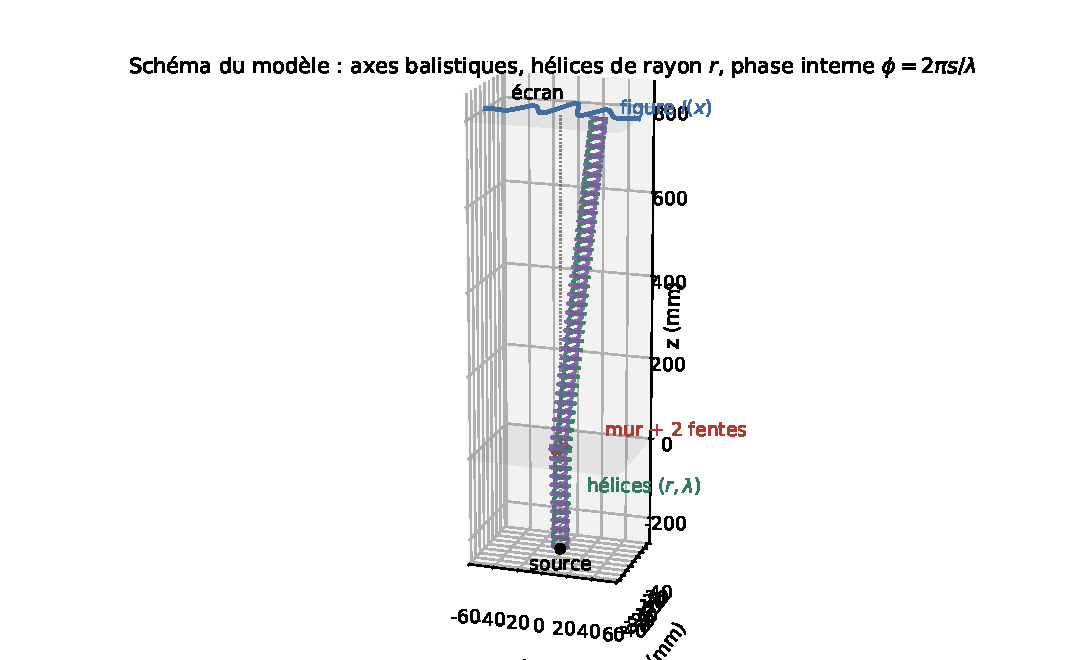
\includegraphics[width=0.84\textwidth]{figures/fig_principe.pdf}
  \caption{Schéma du modèle (échelle non contractuelle). Chaque corpuscule suit
  un axe balistique (pointillés) autour duquel il décrit une hélice de rayon $r$
  et de pas $\lambda$ portant sa phase interne $\phi = 2\pi s/\lambda$. Le point
  réel de l'hélice teste le mur (fente ou paroi) ; à l'arrivée, la détection est
  modulée par le facteur $G(x)$ construit sur les chemins virtuels des $N$ fentes,
  ce qui peint la figure d'interférence $I(x)$ sur l'écran.}
  \label{fig:principe}
\end{figure}

\begin{figure}[t]
  \centering
  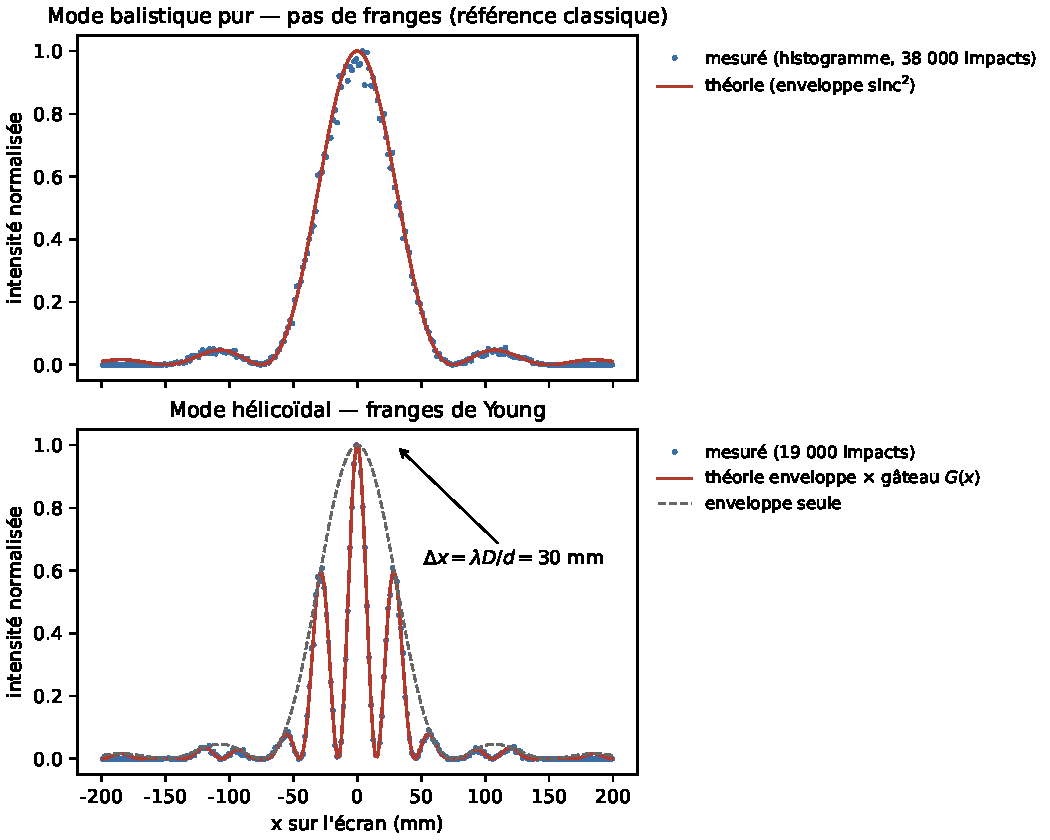
\includegraphics[width=0.88\textwidth]{figures/fig_balistique_helicoide.pdf}
  \caption{Mesures batch sur le noyau exact du simulateur (points : histogrammes
  d'impacts ; courbes : théorie du modèle, sans ajustement). \textbf{Haut} :
  mode balistique pur, $1{,}2\times10^5$ émissions, $37\,975$ impacts --- deux
  taches de diffraction, modulation $M = 0{,}004$ : aucune frange.
  \textbf{Bas} : mode hélicoïdal, $1{,}2\times10^5$ émissions, $19\,025$ impacts
  --- les franges de Young apparaissent avec $M = 0{,}994$ ; l'enveloppe seule
  (tirets) rappelle la référence balistique.}
  \label{fig:balhel}
\end{figure}

La figure~\ref{fig:balhel} porte le résultat central. En mode balistique pur ---
corpuscules ponctuels sur axes classiques, divergence de Fraunhofer au passage des
fentes --- l'histogramme d'impacts reproduit exactement la prédiction classique :
deux taches de diffraction et \emph{aucune frange}, modulation
$M = 0{,}004 \pm$ bruit de comptage. En mode hélicoïdal --- mêmes axes, mêmes
corpuscules, munis de leur phase interne et du facteur de détection $G(x)$ ---
les franges de Young apparaissent : $M = 0{,}994$. Entre les deux modes, la seule
différence est la phase interne portée par l'hélice : ni superposition d'états,
ni interaction entre corpuscules, ni onde externe.

Trois vérifications quantitatives indépendantes accompagnent cette image.
D'abord l'écart de frange : la valeur de $\dx$ qui maximise la modulation
mesurée est $\dx = 30{,}15$~mm, contre $30{,}0$~mm pour la théorie
$\lambda D /d$ --- un accord à $0{,}5\,\%$, sans paramètre ajusté. Ensuite la
fraction détectée : sur $37\,894$ corpuscules parvenus à l'écran en mode
hélicoïdal, $19\,025$ sont détectés et $18\,869$ rejetés par le gâteau, soit une
fraction détectée de $50{,}21\,\%$ contre la prédiction $\langle G \rangle = 1/N
= 50\,\%$ : le modèle est cohérent avec sa propre statistique à $0{,}2\,\%$
près. Enfin le flux : la part du faisceau qui franchit le mur vaut $31{,}6\,\%$
mesurée contre $32\,\%$ géométrique ($2 \times 1{,}6$~mm de fentes ouvertes sur
$10$~mm de faisceau) ; les $81\,713$ photons absorbés ($68{,}1\,\%$ du faisceau)
sont comptés et visibles en tant qu'éclats sur le mur dans le simulateur.

\subsection{La figure se construit corpuscule après corpuscule}

\begin{figure}[t]
  \centering
  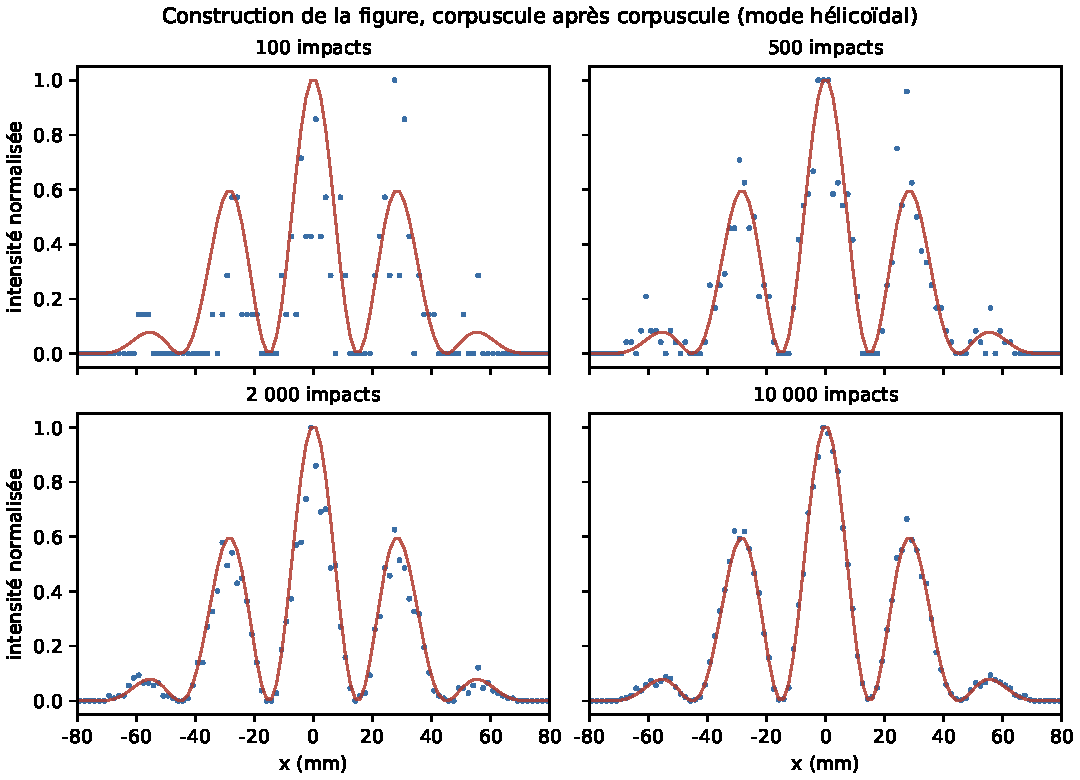
\includegraphics[width=0.95\textwidth]{figures/fig_emergence.pdf}
  \caption{Émergence de la figure (mode hélicoïdal). Clichés de l'histogramme
  d'impacts après $100$, $500$, $2\,000$ et $10\,000$ détections (points), la
  courbe théorique étant inchangée. Chaque impact individuel paraît aléatoire ;
  la distribution ne se distingue du régime balistique qu'après quelques centaines
  d'impacts, et les franges sont nettes vers $10^4$ détections --- l'analogue
  exact du film de Tonomura \cite{tonomura1989}.}
  \label{fig:emergence}
\end{figure}

La figure~\ref{fig:emergence} répond à la question « particule après
particule ». À $100$ impacts, l'histogramme est un semis apparemment désordonné
--- chaque corpuscule individualisé se comporte en tous points comme une particule
classique traverse une fente bien définie. À $10^4$ impacts, les franges sont
constituées. Il n'existe \emph{aucune étape intermédiaire} où deux corpuscules
auraient interagi : chacun ne « voit » que le mur, les fentes et l'écran. C'est la
réplique quantitative de l'expérience de Tonomura \cite{tonomura1989}, et
l'argument le plus direct contre tout mécanisme de franges par interaction
inter-corpuscules.

\subsection{Variantes : mono-fente, photon contre massif, collisions}

\begin{figure}[t]
  \centering
  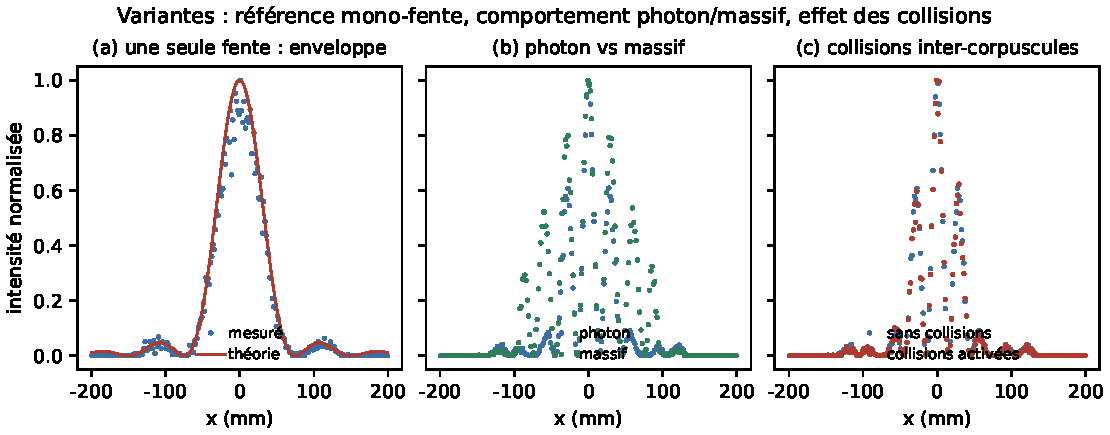
\includegraphics[width=0.98\textwidth]{figures/fig_variantes.pdf}
  \caption{Trois variantes du protocole. \textbf{(a)} Une seule fente ouverte
  ($6\times10^4$ émissions) : l'enveloppe seule, $M = 0{,}022$ --- le modèle
  retrouve automatiquement qu'une fente unique ne frange pas, car $G=1$ dès que
  $N=1$. \textbf{(b)} Photon (bleu) contre corpuscule massif (vert) : le photon
  est absorbé par la paroi ($81\,713$ absorptions, pas de halo), le massif est
  diffusé par les arêtes ($40\,732$ diffusions) et ajoute un fond diffus large,
  tandis que les franges centrales subsistent ($M = 0{,}99$).
  \textbf{(c)} Collisions inter-corpuscules activées (rayon $2$~mm, débit
  quadruplé) : $1\,355$ collisions enregistrées, $M$ passe de $0{,}994$ à
  $0{,}981$.}
  \label{fig:variantes}
\end{figure}

La figure~\ref{fig:variantes} teste trois conclusions structurelles du modèle.
\emph{(a) Mono-fente.} Avec une seule fente, $N=1$ dans l'équation~\eqref{eq:gateau}
donne $G \equiv 1$ : le modèle prédit l'enveloppe de diffraction seule, sans
franges, sans qu'on lui ait rien demandé --- et c'est ce que la mesure donne
($M = 0{,}022$). La structure multi-fentes du facteur de détection est donc bien
la seule source de franges. \emph{(b) Photon contre massif.} Le photon absorbé
par la paroi disparaît proprement : la figure reste franche, sans halo. Le
corpuscule massif, lui, est dévié par les arêtes ($40\,732$ diffusions sur
$6\times10^4$ émissions, soit $67{,}9\,\%$ du faisceau) : il survit et sème un
fond diffus sur tout l'écran, tout en laissant les franges centrales intactes
($M = 0{,}99$ contre $0{,}994$ pour le photon). Les deux comportements demandés
--- absorption franche pour le photon, déviation diffuse pour le massif --- sont
donc obtenus sans contaminer la figure d'interférence. \emph{(c) Collisions.}
Avec les collisions activées (sphères dures élastiques entre points réels des
hélices, rayon $2$~mm, $400$ corpuscules simultanés en vol), $1\,355$ collisions
sont comptées et la modulation \emph{recule} : $M = 0{,}981$ contre $0{,}994$
sans collisions. La dégradation est modeste à cette densité, mais elle est
systématique et \emph{jamais inversée} : dans ce simulateur, ajouter des
interactions entre corpuscules n'a jamais construit une frange --- elles
n'ont d'autre effet que d'éparpiller. C'est la contre-épreuve quantitative de la
section~\ref{sec:intro} : le mécanisme des franges est interne au corpuscule, et
les collisions ne font que brouiller.

\subsection{Évolution d'amplitude : franges étirées, $z$ effectif}

\begin{figure}[t]
  \centering
  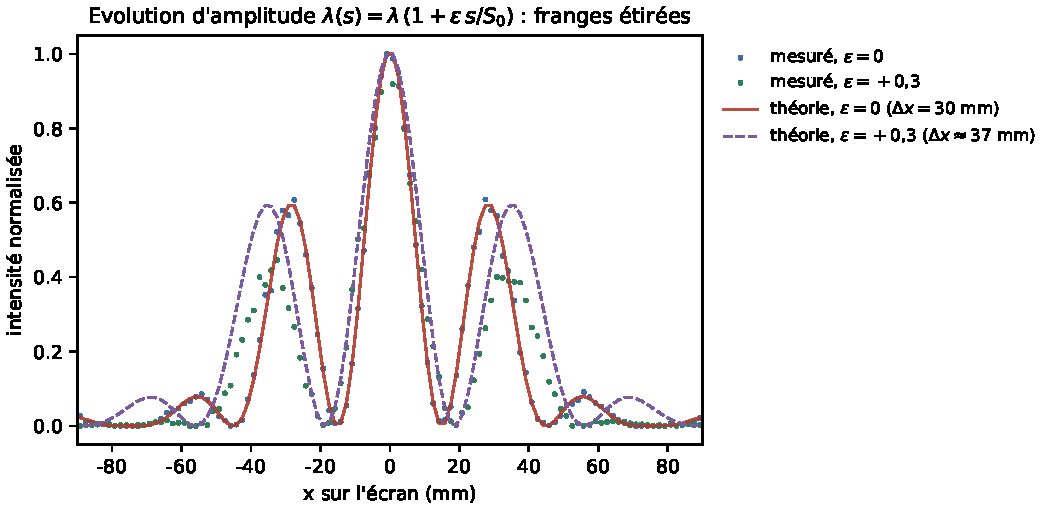
\includegraphics[width=0.88\textwidth]{figures/fig_redshift.pdf}
  \caption{Étude « redshift » ($6\times10^4$ émissions). Points bleus :
  référence $\varepsilon = 0$ ; points verts : $\varepsilon = +0{,}3$, c'est-à-dire
  $z_{\mathrm{eff}} = \varepsilon D/S_0 = 0{,}24$ et $\lambda_{\mathrm{eff}} =
  1{,}24\,\lambda$. Courbes : théorie du modèle aux mêmes paramètres. L'écart de
  frange mesuré passe de $30{,}15$~mm à $37{,}4$~mm, contre $37{,}2$~mm attendus
  ($+0{,}5\,\%$) : les franges sont étirées exactement comme le ferait un
  décalage spectral de facteur $1+z_{\mathrm{eff}}$, alors que l'énergie portée
  par chaque corpuscule est inchangée.}
  \label{fig:redshift}
\end{figure}

La figure~\ref{fig:redshift} applique la loi d'évolution d'amplitude
$\lambda(s) = \lambda(1 + \varepsilon s/S_0)$ avec $\varepsilon = +0{,}3$. Le
décalage effectif simulé vaut $z_{\mathrm{eff}} = \varepsilon D/S_0 = 0{,}24$ ;
l'écart de frange mesuré passe de $30{,}15$~mm (référence) à $37{,}4$~mm, contre
$37{,}2$~mm attendus par la longueur d'onde effective à l'écran. La structure
des franges est donc étirée du facteur $1+z_{\mathrm{eff}}$ exactement comme si
le spectre avait été décalé --- mais aucun corpuscule n'a perdu d'énergie en
chemin : seule l'horloge interne a glissé, conformément à la
loi~\eqref{eq:phaseL}. La fraction détectée reste $50{,}0\,\%$
($9\,509$ détectés, $9\,506$ rejetés) : l'étirement de phase ne change pas le
budget de détection, indice que le flux total est conservé dans le jouet
numérique. Ce point structurel --- un décalage \emph{sans perte d'énergie} ---
est le cœur de la discussion cosmologique de la section~\ref{sec:redshift}.

\begin{table}[t]
\centering\small
\caption{Récapitulatif des six runs batch (paramètres du
tableau~\ref{tab:params} sauf indication). $M$ : modulation de
frange~\eqref{eq:M} ; $\dx$ : écart de frange mesuré par maximisation de $M$
(valeur théorique entre parenthèses).}
\label{tab:runs}
\begin{tabular}{@{}l r r c l l@{}}
\toprule
Run & Émises & Détectées & $M$ & $\dx$ mesuré & Note \\
\midrule
Balistique pur   & $120\,000$ & $37\,975$ & $0{,}004$ & --- & enveloppe seule \\
Hélicoïdal       & $120\,001$ & $19\,025$ & $0{,}994$ & $30{,}15$ ($30{,}0$) & franges \\
Mono-fente       & $60\,007$  & $9\,135$  & $0{,}022$ & --- & enveloppe seule \\
Massif           & $60\,000$  & $29\,703$ & $0{,}99$  & --- & halo de diffusion \\
Redshift $\varepsilon = 0{,}3$ & $60\,002$ & $9\,509$ & $1{,}00$ & $37{,}4$ ($37{,}2$) & $z_{\mathrm{eff}} = 0{,}24$ \\
Collisions       & $60\,001$  & $8\,944$  & $0{,}981$ & --- & $1\,355$ collisions \\
\bottomrule
\end{tabular}
\end{table}

% ============================================================
\section{Lien avec le spin : la zitterbewegung}\label{sec:spin}
% ============================================================

La lecture « hélice interne $\leftrightarrow$ spin » a une histoire précise.
Schrödinger découvre dès 1930, dans les solutions de l'équation de Dirac, une
oscillation interne de l'électron à la fréquence $2mc^2/h$, la
\emph{zitterbewegung} \cite{schrodinger1930}. Hestenes propose en 1990 d'en faire
la clé de voûte de l'interprétation : l'électron y est une charge ponctuelle
décrivant une \emph{hélice} de rayon
\begin{equation}\label{eq:rz}
  r_z \;=\; \frac{\hbar}{2mc} \;=\; \frac{\hbar}{m c}\,\frac{1}{2},
\end{equation}
enroulée autour de la ligne d'univers parcourue à la vitesse moyenne de la
particule \cite{hestenes1990}. Le spin n'y est pas une propriété primitive : il
est le \emph{moment orbital du mouvement circulaire interne},
\begin{equation}\label{eq:spin}
  \lVert \vec S \rVert \;=\; m\,c\,r_z \;=\; \frac{\hbar}{2},
\end{equation}
et le moment magnétique suit, puisque la charge tournante boucle avec elle. Le
sens d'enroulement fixe l'orientation du spin.

Le simulateur de cet article est le banc d'essai minimal de cette famille
d'idées, débarrassé de la dynamique de Dirac : un corpuscule, une hélice de
rayon $r$ et de pas $\lambda$, une phase interne qui tourne comme $2\pi s/
\lambda$ --- l'« horloge interne » que de Broglie postulait dès 1927 comme
phénomène périodique au cœur du corpuscule \cite{debroglie1927} --- et un sens
d'enroulement (le paramètre \emph{spin} $\pm 1$ du simulateur, qui inverse le sens
de rotation de $\phi$). Ce que la section~\ref{sec:res} établit est précisément
le minimum dont l'interprétation zitter a besoin pour être \emph{cohérente avec
l'expérience} : une phase interne portée par le mouvement hélicoïdal suffit
statistiquement à produire la figure d'interférence, sans onde-pilote externe et
sans interaction entre corpuscules. En ce sens, le résultat du présent travail
est compatible avec, et fournit un jouet quantitatif pour, l'identification
hélice~$\leftrightarrow$~zitterbewegung~$\leftrightarrow$~spin.

Il faut être strict sur ce que le simulateur ne montre pas. D'abord,
l'échelle : $r_z = \hbar/2mc$ vaut $1{,}9\times10^{-13}$~m pour l'électron, là
où le simulateur travaille à $r = 0{,}35$~mm --- l'identification est
structurelle, l'échelle étant normalisée (section~\ref{sec:limites}).
Ensuite, la dynamique : le simulateur n'implémente pas l'équation de Dirac, ne
dérive ni le facteur gyromagnétique, ni la statistique fermionique, ni les états
de spin superposés ; le « spin » du simulateur est un sens de rotation classique.
Enfin, pour le photon, l'analogue n'est pas la zitterbewegung mais
l'\emph{hélicité} : une polarisation circulaire porte déjà un moment angulaire
$\pm\hbar$ le long de la propagation, et il n'existe pas de formulation établie
d'un photon localisé sur trajectoire hélicoïdale ; le simulateur traite donc le
photon par la seule hélice de phase, sans prétendre modéliser sa polarisation.
La position honnête est la suivante : le simulateur \emph{supporte} la
compatibilité de l'hypothèse (une phase hélicoïdale interne reproduit Young), il
ne l'\emph{établir} pas.

% ============================================================
\section{Piste de décalage vers le rouge par évolution d'amplitude}\label{sec:redshift}
% ============================================================

\subsection{Ce que la loi $\varepsilon$ réalise dans le simulateur}

Avec $\varepsilon \ne 0$, la phase cumulée $\Phi(L)$ cesse d'être linéaire
(équation~\eqref{eq:phaseL}) : tout se passe, du seul point de vue de la figure
d'interférence, comme si la longueur d'onde glissait de $\lambda$ à
$\lambda(1 + \varepsilon L/S_0)$ le long du trajet. Le simulateur mesure alors,
propagation après propagation, un décalage spectral \emph{apparent} de facteur
$1 + z_{\mathrm{eff}}$ avec $z_{\mathrm{eff}} = \varepsilon\,D/S_0$
--- linéaire en $D$, comme la loi de Hubble l'est en première approximation.
La section~\ref{sec:res} a vérifié quantitativement ce comportement
($37{,}4$~mm mesurés contre $37{,}2$~mm attendus à $z_{\mathrm{eff}} = 0{,}24$).
La question qui intéresse la cosmologie est : \emph{qu'est-ce qui distingue
structurellement ce « décalage de phase » de la « lumière fatiguée » ?}

\subsection{Distinction d'avec la lumière fatiguée de Zwicky}

La lumière fatiguée suppose que le photon \emph{perd de l'énergie} en chemin
\cite{zwicky1929} ; trois familles d'observations l'ont discréditée. Le test de
Tolman : dans un univers sans expansion, la brillance de surface des galaxies ne
peut décroître qu'en $(1+z)^{-2}$ (dilution géométrique), alors que
l'expansion prédit --- et l'observation confirme --- une décroissance proche de
$(1+z)^{-4}$ \cite{lubin2001}. La dilatation temporelle : les courbes de lumière
des supernovae Ia sont observées étirées du facteur $(1+z)$
\cite{leibundgut1996}, ce qu'un photon qui « fatigue » ne produit pas. L'absence
de flou : une perte d'énergie par diffusion élargit les images, non observées.

La variante « évolution d'amplitude » a un profil différent, et c'est ce qui
justifie de l'étudier séparément plutôt que de la rejeter par le label
« lumière fatiguée » :
\begin{itemize}[leftmargin=1.6em,itemsep=0.15em]
  \item \textbf{Pas de perte d'énergie}. Le corpuscule arrive avec l'énergie avec
        laquelle il est parti ; seul le pas de son horloge interne a glissé. La
        relation précise entre ce pas interne et la fréquence spectroscopiquement
        mesurée est une hypothèse à construire, non un acquis --- le simulateur
        est volontairement agnostique ici.
  \item \textbf{Pas de flou}. Aucune diffusion n'accompagne le glissement de
        phase : les images lointaines ne seraient pas élargies par le mécanisme
        lui-même (le simulateur le confirme : la finesse des franges est
        conservée à $\varepsilon$ non nul, $M = 1{,}00$).
  \item \textbf{Dilatation temporelle structurelle}. Si tout processus
        périodique de la source est indexé sur la phase interne du corpuscule,
        alors l'étirement des échelles de temps observées par le facteur
        $(1+z)$ est \emph{automatique} dans cette famille d'hypothèses : la
        dilatation temporelle des supernovae Ia cesse d'être un obstacle pour
        devenir une conséquence qualitative.
  \item \textbf{Le test de Tolman demeure l'obstacle central}. Le budget de
        détection du simulateur est insensible à $\varepsilon$ (fraction
        détectée $50{,}0\,\%$ à $\varepsilon = 0$ comme à $0{,}3$) : à ce niveau
        du jouet, rien ne fournit le facteur $(1+z)^{-4}$ de brillance de
        surface. Toute variante sérieuse devra soit l'engendrer, soit en
        rendre compte autrement ; c'est le test que le paramètre $\varepsilon$
        permet de formuler en laboratoire numérique.
\end{itemize}

\subsection{Échelle de l'analogie, et programme}

L'analogie est structurelle, pas quantitative. Le taux de glissement du
simulateur vaut $\varepsilon/S_0 = 3\times10^{-4}$~mm$^{-1}$ pour obtenir
$z_{\mathrm{eff}} = 0{,}24$ sur $D = 800$~mm. Le taux qui reproduirait la loi de
Hubble ($z \approx H_0 D/c$) vaut $H_0/c \approx 8\times10^{-27}$~m$^{-1}$
($H_0 \approx 70$~km/s/Mpc) : plus de vingt-cinq ordres de grandeur séparent le jouet
numérique de la moindre prétention cosmologique directe. Le rôle du simulateur
n'est pas de « faire de la cosmologie », mais d'offrir la première maquette
contrôlée du mécanisme : une commande numérique $\varepsilon$, une mesure
d'étirement, un budget d'énergie et de flux comptés --- sur lesquels on peut
greffer, étape par étape, les tests que toute variante réelle devra affronter :
linéarité $z(D)$, dilatation temporelle, finesse des images, brillance de
surface, et compatibilité avec le spectre du fond diffus cosmologique (un
étirement uniforme de toutes les longueurs d'onde préserve la forme du spectre
de Planck, ce qui est en revanche un critère redoutable pour tout mécanisme
sélectif en énergie).

% ============================================================
\section{Limites déclarées}\label{sec:limites}
% ============================================================

Le modèle est un instrument de falsification, et ses limites font partie de sa
définition. \textbf{(i)} Le facteur de détection $G(x)$ est \emph{posé},
pas dérivé d'une dynamique : le simulateur mesure sa cohérence statistique
(fraction $1/N$), il ne l'explique pas. \textbf{(ii)} La divergence post-fente
injecte l'enveloppe de Fraunhofer comme loi de tirage : le corpuscule « prend »
l'étalement que la théorie ondulatoire prédit, c'est une correspondance
construite, un paramètre et non un résultat. \textbf{(iii)} L'échelle est
normalisée ($\approx\times1000$) : aucune prétention quantitative sur les hélices
réelles (rayon $\hbar/2mc$ de la zitterbewegung) à ce stade. \textbf{(iv)} Le
comportement « massif » aux arêtes est une diffusion paramétrique, pas un
potentiel de bord dérivé. \textbf{(v)} La statistique d'écran est un empilement
d'événements indépendants : aucun effet de mémoire entre corpuscules,
contrairement aux gouttes marchantes de Couder qui gardent la trace de leur
passage \cite{couder2006,bush2015} --- ce qui, soit dit en passant, est aussi la
raison pour laquelle le simulateur ne peut pas reproduire les phénomnes de
\emph{mémoire} observés dans les analogues hydrodynamiques, et ne le cherche pas.
Enfin, rappelons que la reproduction statistique de Young par une phase interne
n'apporte \emph{aucune} évidence contre la mécanique quantique standard : elle
montre qu'un lagrangien d'information plus pauvre (trajectoire + phase) suffit
pour cette classe d'observations, ce qui est une contrainte de parcimonie sur les
interprétations, pas une réfutation.

% ============================================================
\section{Conclusions}\label{sec:ccl}
% ============================================================

Nous avons construit et validé quantitativement un simulateur stochastique de
l'expérience des fentes de Young dans lequel chaque corpuscule --- photon ou
particule massive --- suit une trajectoire hélicoïdale continue portant une phase
interne, traverse \emph{une} fente à la fois, n'interagit jamais avec ses
congénères, et dont la détection est modulée par un facteur de cohérence de phase
entre les chemins virtuels. Les résultats vont au-delà d'une reproduction
visuelle : l'écart de frange est mesuré à $0{,}5\,\%$ de la théorie
($30{,}15$ contre $30{,}0$~mm), la fraction détectée à $0{,}2\,\%$ de la
prédiction interne ($50{,}21\,\%$ contre $50\,\%$), la modulation de frange passe
de $0{,}004$ (balistique pur) à $0{,}994$ (hélicoïdal), une fente unique
retrouve l'enveloppe seule, le photon est absorbé par la paroi là où le massif
est dévié et sème un halo, les collisions inter-corpuscules ne font que
dégrader la figure, et un glissement d'amplitude $\varepsilon$ étire les franges
exactement comme un décalage spectral sans perte d'énergie ($37{,}4$ contre
$37{,}2$~mm attendus à $z_{\mathrm{eff}} = 0{,}24$).

Deux pistes de recherche en découlent, désormais dotées d'un banc d'essai
public. Pour le \textbf{spin}, le simulateur fournit le socle minimal dont
l'interprétation zitterbewegung de Hestenes a besoin : une phase hélicoïdale
interne reproduit Young ; l'identification à $r_z = \hbar/2mc$ reste qualitative
et cible future. Pour le \textbf{décalage vers le rouge}, la variante
« amplitude glissante » est structurellement distincte de la lumière fatiguée
(énergie conservée, pas de flou, dilatation temporelle automatique), mais elle
doit affronter le test de Tolman, et le simulateur offre la maquette pour
formuler ce test. Tout est reproductible en deux commandes : le code est
distribué (MIT), les mesures exportées (CSV) et chaque figure de cet article
provient du noyau exact du simulateur interactif.

% ============================================================
\appendix
\section{Reproductibilité}\label{sec:repro}
% ============================================================

Le dépôt \texttt{simulation-helicoide} contient les sources complètes. Le livrable
principal est le simulateur autonome \fichierstandalone
(double-clic, hors ligne). Les sources lisibles vivent dans \texttt{src/} :
\texttt{noyau.js} pour la physique, \texttt{rendu.js} pour la scène 3D,
\texttt{interface.js} pour les commandes. Les données exportées vivent dans
\texttt{data/} : histogrammes \texttt{mesures\_*.csv}, compteurs
\texttt{mesures\_resume.json} et métriques \texttt{mesures\_metriques.json}.
Enfin, \texttt{article/} contient la présente prépublication compilable. Les
figures et métriques de la section~\ref{sec:res} se régénèrent par :
\begin{center}\small
\begin{tabular}{@{}l@{\hspace{1.2em}}l@{}}
\texttt{node outils/mesures\_lot.js} & six runs batch ($\approx 5$~s de calcul) \\
\texttt{python3 outils/genere\_figures.py} & figures + métriques JSON \\
\texttt{python3 outils/construire\_standalone.py} & reconstruit le HTML autonome \\
\end{tabular}
\end{center}
Environnement : Node.js $\ge 14$ et Python 3 avec \texttt{numpy} et
\texttt{matplotlib} ; la compilation de l'article requiert Tectonic (LaTeX).
Le générateur de figures lit les CSV de mesures ; la courbe théorique affichée
est celle du modèle (équations~\eqref{eq:gateau}--\eqref{eq:phaseL}) évaluée aux
mêmes paramètres, sans ajustement. Licences : code et simulateur sous MIT,
documentation et article sous CC~BY~4.0 ; l'article cite le DOI du dépôt de
code lorsque celui-ci est archivé (Zenodo via GitHub, recommandé).

\begingroup
\setlength{\parskip}{0pt}
\begin{thebibliography}{99}\small
\setlength{\itemsep}{0.15em}

\bibitem{taylor1909}
G.~I. Taylor,
« Interference fringes with feeble light »,
\emph{Mathematical Proceedings of the Cambridge Philosophical Society} \textbf{15},
114--115 (1909).

\bibitem{merli1976}
P.~G. Merli, G.~F. Missiroli, G. Pozzi,
« On the statistical aspect of electron interference phenomena »,
\emph{American Journal of Physics} \textbf{44}, 306--307 (1976).

\bibitem{tonomura1989}
A. Tonomura, J. Endo, T. Matsuda, T. Kawasaki, H. Ezawa,
« Demonstration of single-electron buildup of an interference pattern »,
\emph{American Journal of Physics} \textbf{57}, 117--120 (1989),
\href{https://doi.org/10.1119/1.16104}{doi:10.1119/1.16104}.

\bibitem{bach2013}
R. Bach, D. Pope, S.-H. Liou, H. Batelaan,
« Controlled double-slit electron diffraction »,
\emph{New Journal of Physics} \textbf{15}, 033018 (2013),
\href{https://doi.org/10.1088/1367-2630/15/3/033018}{doi:10.1088/1367-2630/15/3/033018}.

\bibitem{debroglie1927}
L. de Broglie,
onde-pilote et théorie de la double solution,
communications au Congrès Solvay, Bruxelles (1927).

\bibitem{bohm1952}
D. Bohm,
« A suggested interpretation of the quantum theory in terms of ``hidden''
variables. I--II »,
\emph{Physical Review} \textbf{85}, 166--193 (1952).

\bibitem{couder2006}
Y. Couder, E. Fort,
« Single-particle diffraction and interference at a macroscopic scale »,
\emph{Physical Review Letters} \textbf{97}, 154101 (2006),
\href{https://doi.org/10.1103/PhysRevLett.97.154101}{doi:10.1103/PhysRevLett.97.154101}.

\bibitem{eddi2009}
A. Eddi, E. Fort, F. Moisy, Y. Couder,
« Unpredictable tunneling of a classical wave-particle »,
\emph{Physical Review Letters} \textbf{102}, 240401 (2009).

\bibitem{andersen2014}
A. Andersen \emph{et al.},
commentaire sur « Single-particle diffraction and interference at a macroscopic
scale », arXiv:1405.0466 (2014).

\bibitem{bush2015}
J.~W.~M. Bush,
« Pilot-wave hydrodynamics »,
\emph{Annual Review of Fluid Mechanics} \textbf{47}, 269--292 (2015).

\bibitem{schrodinger1930}
E. Schrödinger,
« Über die kräftefreie Bewegung in der relativistischen Quantenmechanik »,
\emph{Sitzungsberichte der Preußischen Akademie der Wissenschaften} (1930).

\bibitem{hestenes1990}
D. Hestenes,
« The zitterbewegung interpretation of quantum mechanics »,
\emph{Foundations of Physics} \textbf{20}, 1213--1232 (1990),
\href{https://doi.org/10.1007/BF01889466}{doi:10.1007/BF01889466}.

\bibitem{zwicky1929}
F. Zwicky,
« On the redshift of spectral lines through interstellar space »,
\emph{Proceedings of the National Academy of Sciences} \textbf{15}, 773--779 (1929),
\href{https://doi.org/10.1073/pnas.15.10.773}{doi:10.1073/pnas.15.10.773}.

\bibitem{lubin2001}
L.~M. Lubin, A. Sandage,
« The Tolman surface brightness test for the reality of the expansion »,
\emph{Astronomical Journal} \textbf{122}, 1084 (2001),
arXiv:astro-ph/0106566.

\bibitem{leibundgut1996}
B. Leibundgut \emph{et al.},
« Time dilation in the light curve of the distant type Ia supernova SN~1995K »,
\emph{Astrophysical Journal (Letters)} \textbf{466}, L21 (1996),
\href{https://doi.org/10.1086/310164}{doi:10.1086/310164}.

\end{thebibliography}
\endgroup

\end{document}
